\documentclass[UTF8,zihao=-4,a4paper]{ctexart}

\usepackage[margin=2.6cm]{geometry}
\usepackage{amsmath,amssymb,bm}
\usepackage{booktabs,threeparttable,longtable,array,tabularx}
\usepackage{graphicx,float,caption,subcaption}
\usepackage{setspace,fancyhdr}
\usepackage{xcolor}
\usepackage{hyperref}
\usepackage[nameinlink,noabbrev]{cleveref}
\usepackage[backend=biber,style=gb7714-2015,sorting=none]{biblatex}
\addbibresource{references.bib}

\hypersetup{
  colorlinks=true,
  linkcolor=black,
  citecolor=blue!55!black,
  urlcolor=blue!55!black,
  pdftitle={中东冲突对国际油价冲击：事件研究法与回归分析}
}
\crefname{table}{表}{表}
\crefname{figure}{图}{图}
\crefname{equation}{式}{式}
\graphicspath{{../figures/}}
\captionsetup{font=small,labelsep=quad}
\setstretch{1.35}
\setlength{\parindent}{2em}
\setlength{\parskip}{0pt}
\ctexset{
  section={format=\Large\bfseries,beforeskip=1.8ex,afterskip=1.0ex},
  subsection={format=\large\bfseries,beforeskip=1.4ex,afterskip=0.8ex}
}
\pagestyle{fancy}
\setlength{\headheight}{15pt}
\fancyhf{}
\fancyhead[C]{数理统计课程大作业}
\fancyfoot[C]{\thepage}
\renewcommand{\headrulewidth}{0.4pt}
\newcommand{\OilSampleN}{345}
\newcommand{\ReturnCorrelation}{0.845}
\newcommand{\EventCount}{5}


\begin{document}

\hypersetup{pageanchor=false}
\begin{titlepage}
  \centering
  \vspace*{1.2cm}
  {\zihao{2}\bfseries 北京航空航天大学\par}
  \vspace{0.7cm}
  {\zihao{3}\bfseries 数理统计课程大作业\par}
  \vspace{2.2cm}
  {\zihao{1}\bfseries 中东冲突对国际油价冲击\par}
  \vspace{0.4cm}
  {\zihao{2}\bfseries ——事件研究法与回归分析\par}
  \vfill
  \renewcommand{\arraystretch}{1.7}
  \begin{tabular}{rl}
    学院： & 人工智能学院 \\
    姓名： & 【请填写姓名】 \\
    学号： & 【请填写学号】 \\
    任课教师： & 【请填写教师姓名】 \\
    提交日期： & 2026年6月 \\
  \end{tabular}
  \vfill
\end{titlepage}

\hypersetup{pageanchor=true}
\pagenumbering{Roman}
\begin{abstract}
本文研究2025年至2026年中东冲突升级对国际原油价格的短期冲击。研究使用FRED口径的WTI与Brent日度价格构造对数收益率，并结合ACLED中东周度汇总数据刻画冲突背景。在对新闻来源进行核验后，选取5个重大事件，采用市场模型估计正常收益，计算$[-1,+1]$、$[0,+3]$与$[0,+5]$三个窗口的累计异常收益（CAR），并实施显著性检验。进一步使用中断时间序列模型（ITS）分解即时水平变化与事件后趋势变化，通过Durbin--Watson检验、Breusch--Pagan检验和Newey--West稳健标准误评估回归推断的可靠性，并采用分段回归与BIC进行结构断点近似识别。

结果表明，不同事件、不同油价基准与不同事件窗口之间存在明显异质性。在主窗口$[0,+3]$中，2026年3月13日哈尔克岛及石油出口设施风险事件对应的Brent CAR为$13.552\%$，WTI相对Brent的CAR为$-10.198\%$；两者在Bonferroni和Benjamini--Hochberg修正后仍显著。ITS结果显示，2026年2月28日冲突升级对Brent收益率产生显著正向水平变化，而结构断点集中出现在2026年2月底至3月初。研究说明，中东冲突并不会机械地导致所有油价基准同向上涨；市场反应取决于事件是否直接威胁供应链、风险是否已被提前定价，以及所使用正常收益基准的含义。

\noindent\textbf{关键词：}中东冲突；国际油价；事件研究法；累计异常收益；中断时间序列；结构断点
\end{abstract}

\newpage
\tableofcontents
\newpage
\pagenumbering{arabic}

\section{引言}

原油既是基础能源商品，也是对地缘政治信息高度敏感的金融资产。中东地区集中了重要的原油生产、出口和海运通道，军事冲突一旦涉及油田、出口终端或霍尔木兹海峡，市场会通过供应中断预期、库存需求和风险溢价迅速调整价格。然而，油价同时受到全球需求、美元、库存、OPEC政策与金融市场风险偏好的影响，因此，事件发生后出现价格涨跌并不能直接证明事件造成了异常冲击。

事件研究法提供了一种可检验的分析框架：先利用事件前样本估计正常收益，再计算事件窗口内实际收益相对于正常收益的偏离。该方法在金融研究中已形成成熟范式\cite{mackinlay1997,brownwarner1985}。本文将其与中断时间序列、稳健标准误和结构断点方法结合，回答三个问题：第一，重大冲突事件后WTI和Brent的异常收益有多大；第二，哪些事件的影响具有统计显著性；第三，在事件密集发生时，能否区分即时冲击、趋势变化与更长期的结构变化。

本文的主要贡献在于：其一，在统一框架下比较多次冲突事件，而不是只研究单次战争爆发；其二，同时报告WTI与Brent，讨论两种基准对中东供应风险的异质性反应；其三，将CAR、ITS、残差诊断与结构断点进行交叉验证；其四，使用ACLED周度汇总数据为事件发生阶段提供独立的冲突强度背景。

\section{文献综述}

油价冲击并非同质。Kilian\cite{kilian2009}指出，供给冲击、全球需求冲击和预防性需求冲击对油价及宏观经济具有不同影响。这一结论提示我们，军事冲突是否触及实际供应链，是解释市场反应的重要条件。Caldara和Iacoviello\cite{caldara2022}构建地缘政治风险指数，系统说明战争威胁和冲突升级会通过不确定性与风险溢价影响经济和金融市场。

在方法上，MacKinlay\cite{mackinlay1997}和Brown、Warner\cite{brownwarner1985}系统阐述了事件研究的估计窗口、异常收益和显著性检验。对于时间序列中已知干预时点的水平与趋势变化，ITS提供了直观的分段回归框架\cite{bernal2017}。当残差存在异方差或自相关时，Newey--West协方差矩阵能够提供更稳健的统计推断\cite{neweywest1987}。对于未知时点的制度变化，Bai--Perron方法则允许在回归模型中识别多个结构断点\cite{bai1998,bai2003}。

现有文献为本文提供了完整的方法基础，但对2025年至2026年伊以及相关冲突中的多事件比较仍较少。本文重点不是构建复杂的预测模型，而是以课程所学的统计推断方法回答“哪些事件显著、冲击有多大、结论是否稳健”。

\section{理论机制与研究假设}

冲突影响油价主要经过三条路径。第一，生产设施受损或制裁升级会降低预期供给；第二，港口、油轮与海峡风险会提高运输成本并增加交割不确定性；第三，即使实际供给尚未中断，市场也可能因预防性库存需求和风险溢价而提前上涨。另一方面，若冲突已被提前计价，或事件后出现停火、增产及需求转弱信息，油价也可能不涨反跌。

据此提出以下研究假设：

\begin{description}
  \item[H1] 重大中东冲突事件会在短期事件窗口内产生显著累计异常收益。
  \item[H2] 相较于WTI，Brent对中东供应与海运风险表现出更强的反应。
  \item[H3] 直接涉及石油出口设施或关键航运通道的事件，其异常收益幅度更大。
\end{description}

\section{数据来源与描述性统计}

\subsection{油价与冲突数据}

WTI和Brent日度价格采用FRED的DCOILWTICO与DCOILBRENTEU口径\cite{fredwti,fredbrent}。共同交易日样本包含\OilSampleN 个观测，主分析覆盖2025年1月1日至2026年6月1日。收益率定义为
\begin{equation}
  r_t=\ln P_t-\ln P_{t-1},
  \label{eq:return}
\end{equation}
其中$P_t$为第$t$个交易日的美元/桶价格。

冲突背景数据来自ACLED中东汇总文件\cite{acleddata}，粒度为“周—国家—一级行政区—事件类型”。本文筛选Iran、Israel、Lebanon、Syria、Iraq和Yemen。该数据用于描述冲突强度和事件周背景，不是逐事件明细，因而不用于替代新闻核验。

\begin{table}[H]
  \centering
  \caption{WTI与Brent日对数收益率描述性统计（单位：\%）}
  \label{tab:desc}
  \small
  \resizebox{\textwidth}{!}{\begin{tabular}{lrrrrrrrr}
\toprule
变量 & $N$ & 均值 & 标准差 & 最小值 & 中位数 & 最大值 & 偏度 & 峰度 \\
\midrule
WTI & 345 & 0.081 & 2.901 & -17.516 & 0.069 & 11.536 & -0.888 & 9.855 \\
Brent & 345 & 0.080 & 2.984 & -16.763 & 0.015 & 11.805 & -0.547 & 8.391 \\
\bottomrule
\end{tabular}
}
  \begin{minipage}{0.95\textwidth}\footnotesize
  注：峰度为非超额峰度，正态分布对应峰度3。WTI与Brent收益率相关系数为\ReturnCorrelation。
  \end{minipage}
\end{table}

由\cref{tab:desc}可见，两种收益率均呈负偏和高峰厚尾特征，峰度显著高于3。这说明极端波动出现概率高于正态分布，使用稳健标准误和多窗口比较具有必要性。两种收益率相关系数为\ReturnCorrelation，表明它们具有较强共同波动，但并非完全同步。

\begin{table}[H]
  \centering
  \caption{目标国家ACLED汇总事件与死亡人数}
  \label{tab:acled-country}
  \begin{tabular}{lrr}
\toprule
国家 & 事件数 & 死亡人数 \\
\midrule
Yemen & 15616 & 3653 \\
Syria & 14663 & 9029 \\
Iran & 12154 & 30638 \\
Lebanon & 11689 & 2985 \\
Iraq & 7518 & 900 \\
Israel & 4298 & 80 \\
\bottomrule
\end{tabular}

  \begin{minipage}{0.85\textwidth}\footnotesize
  注：统计期为2025年1月1日至2026年6月1日；该表为周度聚合数据加总。
  \end{minipage}
\end{table}

\begin{figure}[H]
  \centering
  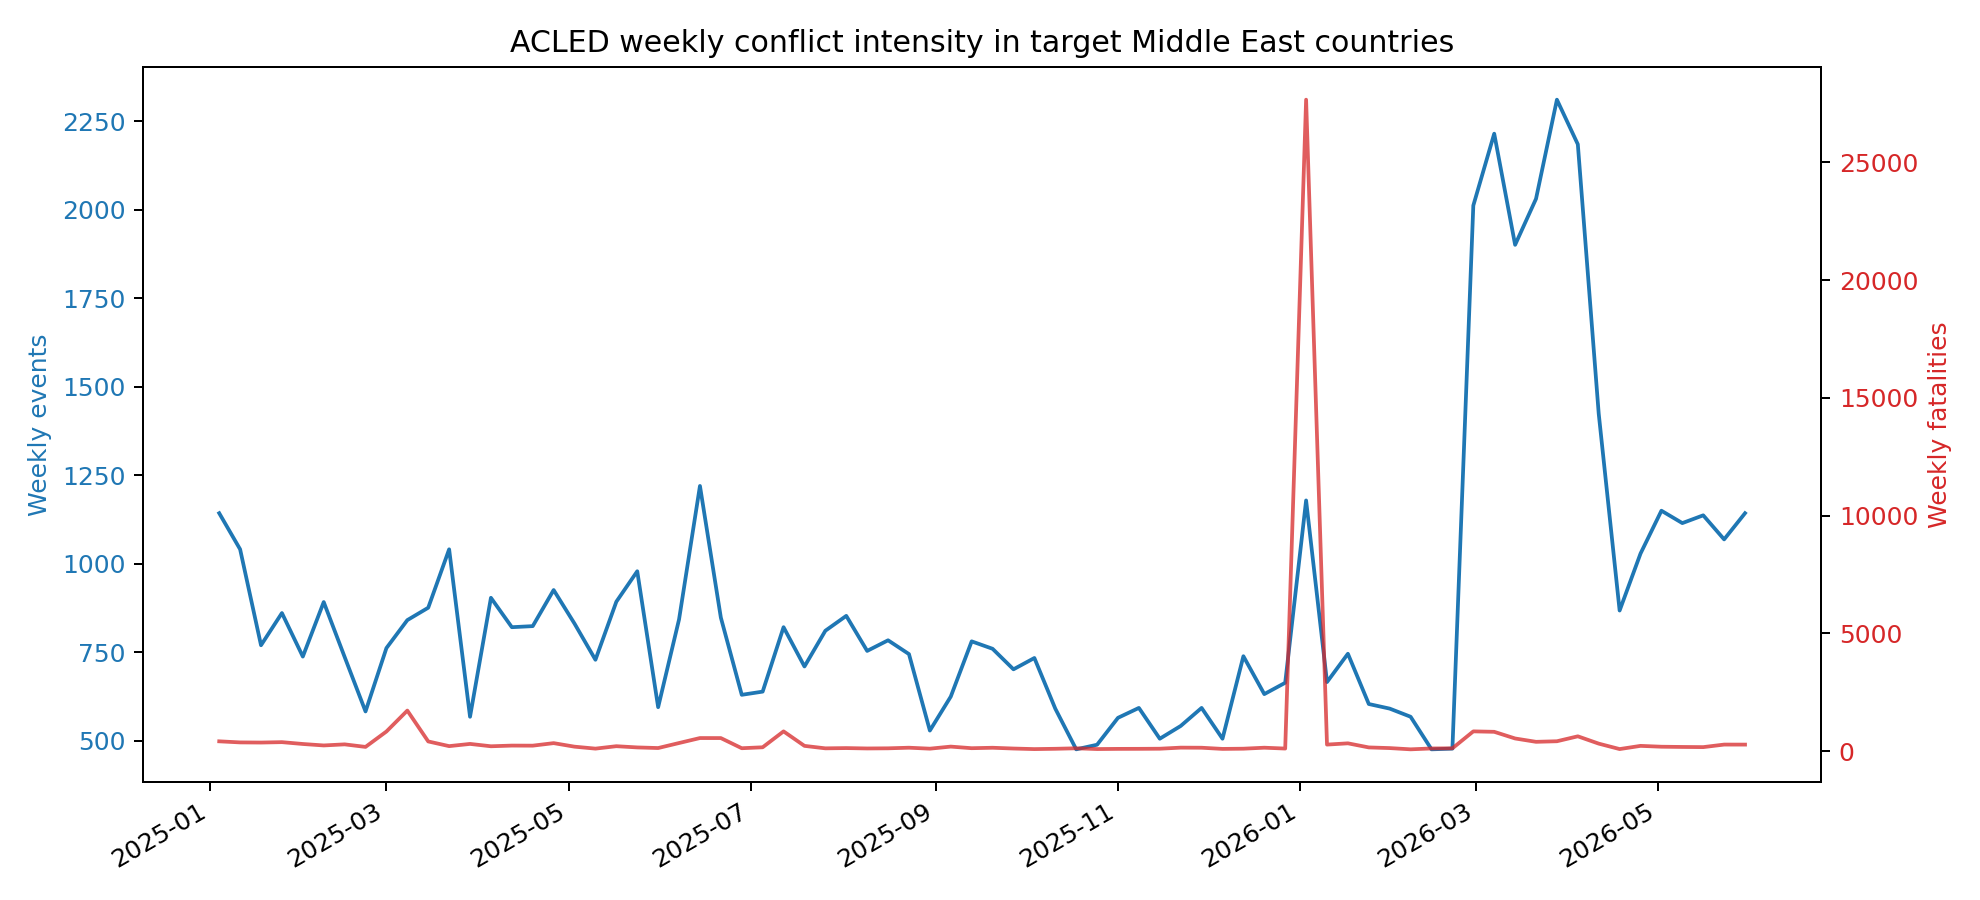
\includegraphics[width=0.96\textwidth]{acled_weekly_events.png}
  \caption{目标国家ACLED周度事件数与死亡人数}
  \label{fig:acled-weekly}
\end{figure}

\section{事件选择与研究设计}

\subsection{事件样本}

事件选择遵循外生信息原则：仅依据公开新闻中的事件日期、事件性质以及其与石油供应链的关联确定，不使用当日油价波动参与筛选。2025年事件由CSIS对以色列打击伊朗及其油市影响的分析核验\cite{csis2025}；2026年2月28日、3月13日和4月13日事件分别由公开新闻来源核验\cite{guardian2026,wpKharg2026,wpBlockade2026}。最终选取\EventCount 个事件，满足作业要求的5至8个事件范围。

\begin{table}[H]
  \centering
  \caption{关键事件及核验来源}
  \label{tab:events}
  \footnotesize
  \resizebox{\textwidth}{!}{\begin{tabular}{lllll}
\toprule
编号 & 事件日期 & 交易日 & 事件说明 & 核验来源 \\
\midrule
E1 & 2025-06-13 & 2025-06-13 & 以色列打击伊朗核设施和军事目标 & CSIS/公开新闻 \\
E2 & 2025-06-17 & 2025-06-17 & 伊以导弹与空袭交锋持续 & CSIS/ACLED周度 \\
E3 & 2026-02-28 & 2026-03-02 & 美以对伊朗发动联合打击 & The Guardian \\
E4 & 2026-03-13 & 2026-03-13 & 哈尔克岛及石油出口设施风险 & Washington Post \\
E5 & 2026-04-13 & 2026-04-13 & 海上封锁与霍尔木兹海峡风险 & Washington Post \\
\bottomrule
\end{tabular}
}
\end{table}

E3发生于周六，因此事件研究将其映射至首个可交易日2026年3月2日。E1与E2仅相隔4天，短窗口可能发生重叠，论文将该问题作为稳健性限制，而不把两次估计解释为完全独立的因果效应。

\begin{table}[H]
  \centering
  \caption{事件间隔与窗口重叠情况}
  \label{tab:overlap}
  \begin{tabular}{llrl}
\toprule
事件 & 日期 & 距上一事件/天 & 五日窗口可能重叠 \\
\midrule
E1 & 2025-06-13 & -- & -- \\
E2 & 2025-06-17 & 4 & 是 \\
E3 & 2026-02-28 & 256 & 否 \\
E4 & 2026-03-13 & 13 & 否 \\
E5 & 2026-04-13 & 31 & 否 \\
\bottomrule
\end{tabular}

\end{table}

\begin{table}[H]
  \centering
  \caption{候选事件所在ACLED周的冲突强度}
  \label{tab:event-week}
  \small
  \resizebox{\textwidth}{!}{\begin{tabular}{lllrrl}
\toprule
事件 & 事件日期 & ACLED周 & 周事件数 & 周死亡数 & 事件最多国家 \\
\midrule
E1 & 2025-06-13 & 2025-06-14 & 1220 & 551 & Iran \\
E2 & 2025-06-17 & 2025-06-21 & 848 & 550 & Yemen \\
E3 & 2026-02-28 & 2026-02-28 & 2012 & 835 & Iran \\
E4 & 2026-03-13 & 2026-03-14 & 1901 & 533 & Iran \\
E5 & 2026-04-13 & 2026-04-18 & 868 & 83 & Iran \\
\bottomrule
\end{tabular}
}
\end{table}

\subsection{正常收益模型与CAR}

以资产$i$的收益率为被解释变量，以另一油价基准收益率为市场参照，估计市场模型
\begin{equation}
  R_{i,t}=\alpha_i+\beta_iR_{m,t}+\varepsilon_{i,t}.
  \label{eq:market}
\end{equation}
估计窗口使用事件日前120个交易日，并与事件日之间保留21个交易日间隔。异常收益与累计异常收益分别为
\begin{align}
  AR_{i,t}&=R_{i,t}-\widehat{R}_{i,t},\\
  CAR_i(\tau_1,\tau_2)&=\sum_{t=\tau_1}^{\tau_2}AR_{i,t}.
  \label{eq:car}
\end{align}
本文使用$[-1,+1]$、$[0,+3]$与$[0,+5]$三个窗口。近似检验统计量为
\begin{equation}
  t=\frac{CAR}{\widehat{\sigma}_{AR}\sqrt{L}},
  \label{eq:tstat}
\end{equation}
其中$L$为事件窗口长度。

需要强调，WTI与Brent互为市场参照意味着本文测量的是一种\textbf{相对异常反应}。若两者同时受到同方向冲击，共同成分会被市场模型部分扣除；若出现相反符号，则应解释为两种基准之间的相对表现，而非原油绝对价格必然反向变化。

\subsection{ITS、稳健标准误与断点识别}

局部中断时间序列模型设为
\begin{equation}
 r_t=\beta_0+\beta_1 time_t+\beta_2 post_t+\beta_3 time\_after_t+\varepsilon_t,
 \label{eq:its}
\end{equation}
其中$\beta_2$刻画即时水平变化，$\beta_3$刻画事件后趋势变化。残差自相关通过Durbin--Watson统计量判断，异方差通过Breusch--Pagan检验判断；最终显著性优先采用Newey--West HAC标准误\cite{neweywest1987}。

结构断点部分采用Bai--Perron思想的简化实现：对所有候选断点进行两段线性回归，依据残差平方和与BIC排序。该方法是单断点网格近似，不等同于正式多断点Bai--Perron检验。

\section{实证结果}

\subsection{主事件窗口结果}

\begin{table}[H]
  \centering
  \caption{主窗口$[0,+3]$的CAR与多重检验修正}
  \label{tab:multiple}
  \small
  \begin{tabular}{llrrrr}
\toprule
基准 & 事件 & CAR(\%) & 原始$p$ & Bonferroni & BH--FDR \\
\midrule
Brent & E1 & 2.265 & 0.1918 & 1.0000 & 0.2741 \\
Brent & E2 & 2.859 & 0.1015 & 1.0000 & 0.2029 \\
Brent & E3 & 2.474 & 0.1585 & 1.0000 & 0.2642 \\
Brent & E4 & 13.552 & 0.0000 & 0.0000 & 0.0000 \\
Brent & E5 & -0.711 & 0.7773 & 1.0000 & 0.9506 \\
WTI & E1 & 0.214 & 0.9092 & 1.0000 & 0.9506 \\
WTI & E2 & -3.681 & 0.0520 & 0.5204 & 0.1735 \\
WTI & E3 & 2.567 & 0.0948 & 0.9476 & 0.2029 \\
WTI & E4 & -10.198 & 0.0000 & 0.0000 & 0.0000 \\
WTI & E5 & -0.165 & 0.9506 & 1.0000 & 0.9506 \\
\bottomrule
\end{tabular}

  \begin{minipage}{0.92\textwidth}\footnotesize
  注：Bonferroni和BH--FDR在主窗口的10个“资产—事件”检验中统一调整$p$值。
  \end{minipage}
\end{table}

\cref{tab:multiple}显示，E4的Brent CAR为$13.552\%$，WTI相对Brent的CAR为$-10.198\%$，两者在多重检验修正后仍显著。这一结果支持H1，也与E4直接涉及伊朗核心出口设施的机制相符，因而为H3提供支持。相较之下，E1、E2与E3在主窗口中的原始$p$值多数处于边际或不显著水平，并且在多重检验修正后不再显著。

E4中两类基准符号相反，不能解读为“冲突使WTI绝对下跌而Brent绝对上涨”的简单因果结论。它更可能反映Brent作为国际海运基准，对中东出口风险的相对反应显著强于WTI。由此，H2在相对反应意义上得到部分支持，但仍需要外部商品指数作为正常收益基准才能得到更强结论。

\begin{figure}[H]
  \centering
  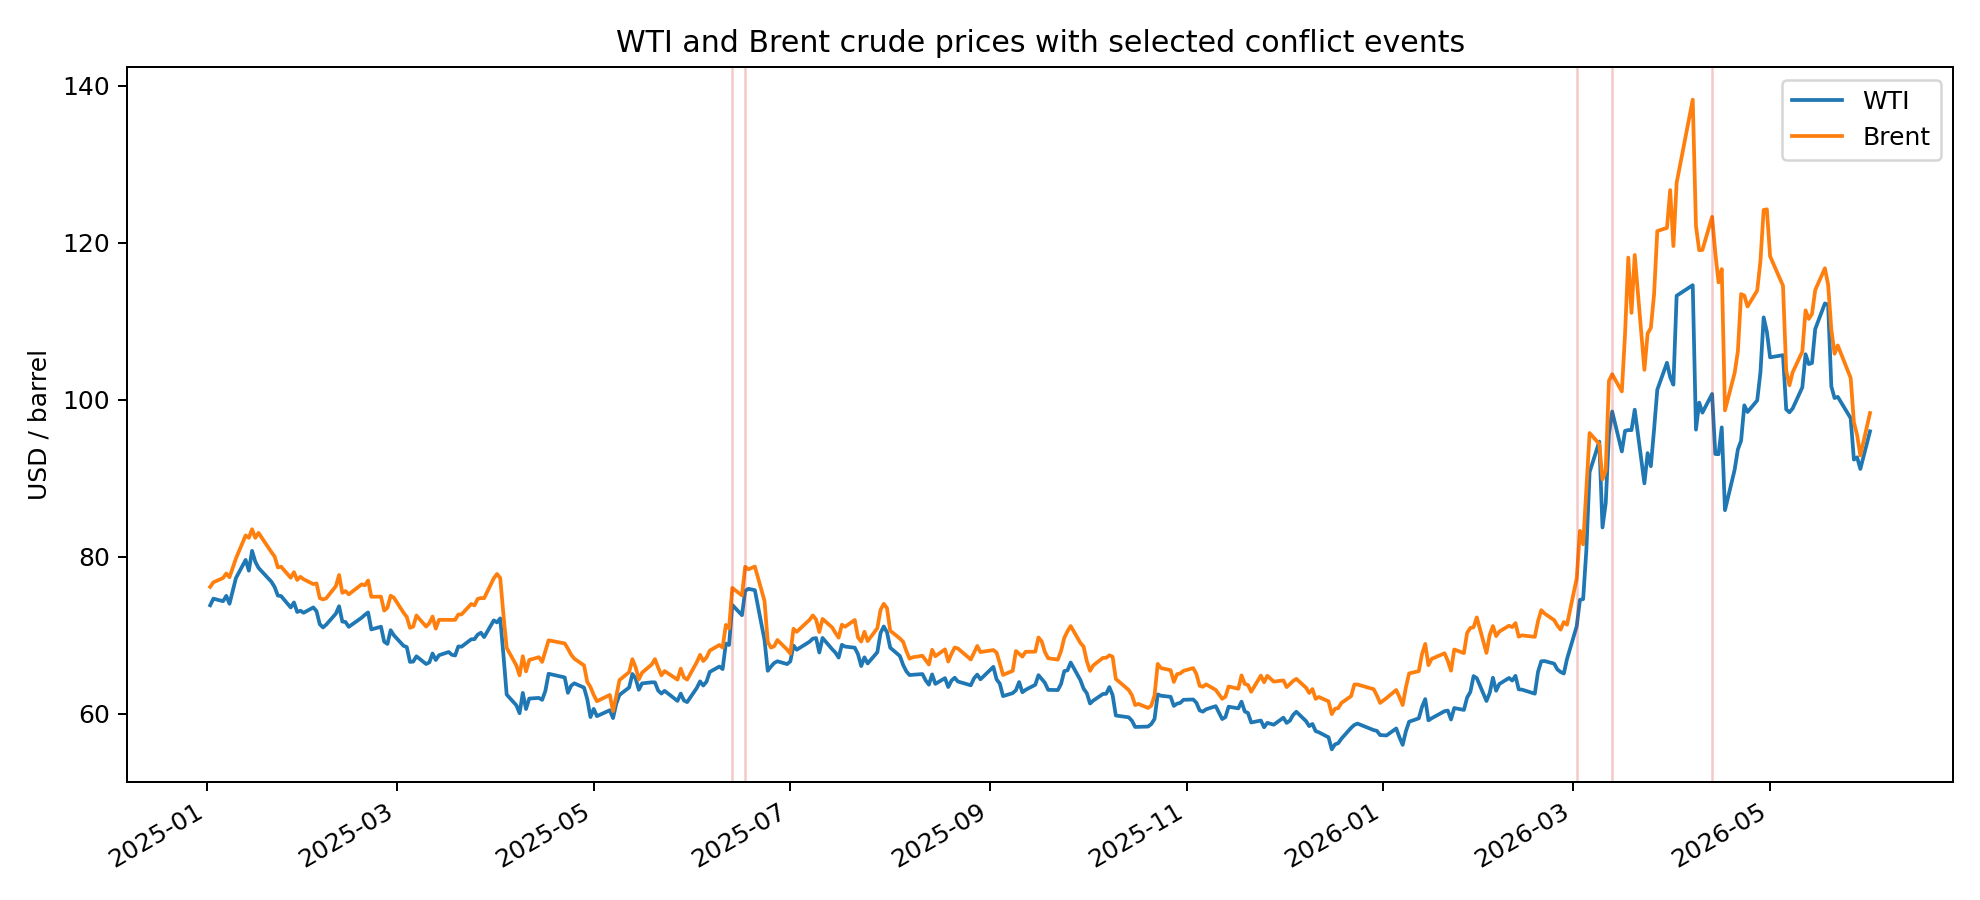
\includegraphics[width=0.96\textwidth]{oil_prices_events.png}
  \caption{WTI、Brent价格与事件日期}
  \label{fig:price}
\end{figure}

\begin{figure}[H]
  \centering
  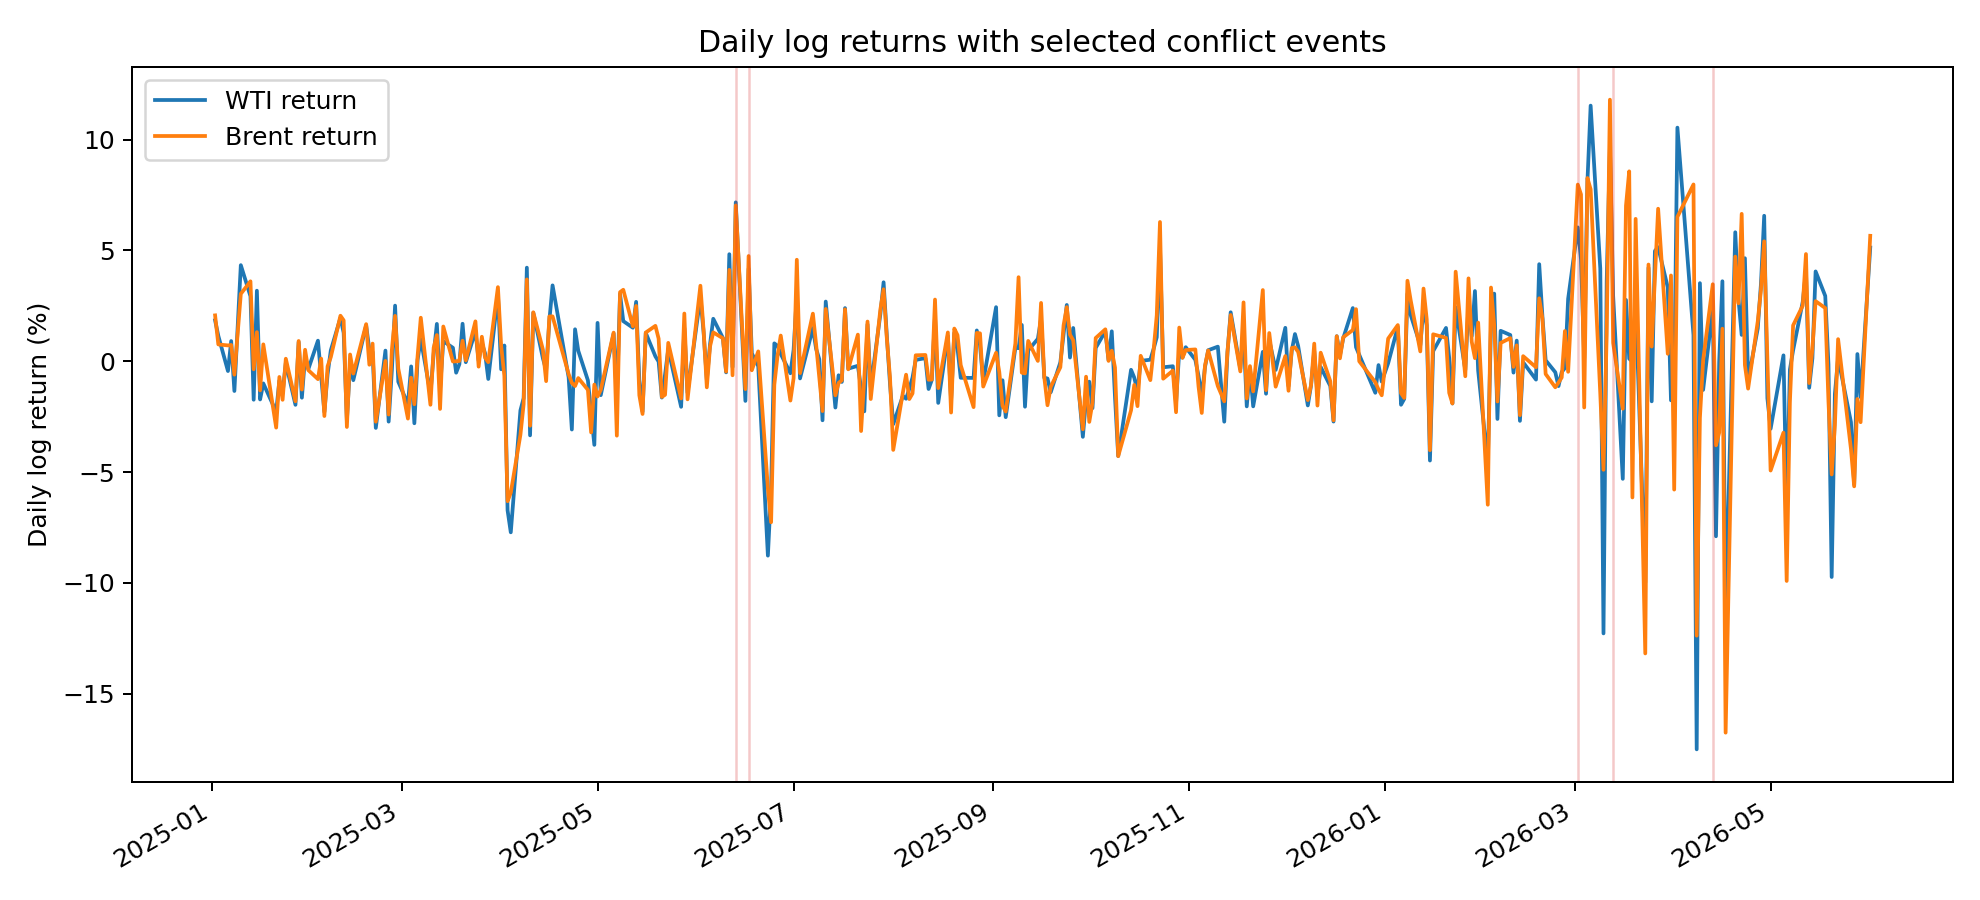
\includegraphics[width=0.96\textwidth]{oil_returns_events.png}
  \caption{WTI、Brent日对数收益率与事件日期}
  \label{fig:return}
\end{figure}

\subsection{ITS与残差诊断}

\begin{table}[H]
  \centering
  \caption{局部ITS、Newey--West修正及残差诊断}
  \label{tab:its}
  \scriptsize
  \resizebox{\textwidth}{!}{\begin{tabular}{llrrrrr}
\toprule
基准 & 事件 & 水平变化(\%) & 趋势变化 & NW $p$ & DW & BP $p$ \\
\midrule
Brent & E1 & -0.488 & -0.0552 & 0.6867 & 1.909 & 0.0026 \\
Brent & E2 & -1.695 & -0.0401 & 0.0818 & 1.961 & 0.0472 \\
Brent & E3 & 3.344 & -0.0795 & 0.0109 & 2.382 & 0.0163 \\
Brent & E4 & -1.796 & -0.1418 & 0.1993 & 2.268 & 0.0528 \\
Brent & E5 & -1.286 & -0.0006 & 0.5206 & 2.148 & 0.1008 \\
WTI & E1 & -0.526 & -0.0461 & 0.6470 & 1.918 & 0.0071 \\
WTI & E2 & -1.597 & -0.0319 & 0.1080 & 1.977 & 0.0697 \\
WTI & E3 & 2.040 & -0.0668 & 0.1656 & 2.199 & 0.0414 \\
WTI & E4 & -3.082 & -0.0915 & 0.0459 & 2.232 & 0.1725 \\
WTI & E5 & 0.071 & 0.0091 & 0.9679 & 2.104 & 0.1339 \\
\bottomrule
\end{tabular}
}
\end{table}

E3后的Brent即时水平变化为$3.344\%$，Newey--West修正后$p=0.0109$；E4后的WTI相对水平变化为$-3.082\%$，修正后$p=0.0459$。多数DW统计量接近2，未显示突出的正向一阶自相关。然而，若干BP检验$p$值低于0.05，说明异方差不可忽略，使用HAC标准误是必要的。

CAR与ITS回答的问题并不完全相同。CAR衡量有限窗口内的累计相对异常收益；ITS中的$\beta_2$衡量事件前后局部收益率水平跳变。两者不一致并不必然代表模型失效，而可能说明冲击以多日累积、提前定价或后续反转的方式体现。

\section{稳健性与结构断点分析}

\subsection{窗口敏感性与多重检验}

完整三个窗口结果见附录\cref{tab:car-all}。部分事件仅在特定窗口显著，说明结论对反应期限敏感。例如，短窗口显著但长窗口不显著，可能意味着风险溢价快速出现后回落；长窗口显著则可能代表供应风险持续发酵。

本文同时报告Bonferroni和BH--FDR修正。Bonferroni控制家族错误率，较为保守；BH--FDR控制错误发现率，更适合同时比较多个事件。在主窗口中，只有E4在两种修正下仍保持显著，说明其证据明显强于其他事件。

\subsection{结构断点}

\begin{table}[H]
  \centering
  \caption{BIC最优结构断点候选}
  \label{tab:breaks}
  \small
  \begin{tabular}{lrllrl}
\toprule
基准 & 排序 & 断点日期 & 最近事件 & 相差天数 & 支持 \\
\midrule
WTI & 1 & 2026-02-27 & 2026-03-02 & 3 & 是 \\
WTI & 2 & 2026-03-02 & 2026-03-02 & 0 & 是 \\
WTI & 3 & 2026-02-26 & 2026-03-02 & 4 & 是 \\
WTI & 4 & 2026-02-25 & 2026-03-02 & 5 & 是 \\
WTI & 5 & 2026-02-18 & 2026-03-02 & 12 & 否 \\
Brent & 1 & 2026-03-02 & 2026-03-02 & 0 & 是 \\
Brent & 2 & 2026-02-27 & 2026-03-02 & 3 & 是 \\
Brent & 3 & 2026-02-26 & 2026-03-02 & 4 & 是 \\
Brent & 4 & 2026-02-25 & 2026-03-02 & 5 & 是 \\
Brent & 5 & 2026-03-03 & 2026-03-02 & 1 & 是 \\
\bottomrule
\end{tabular}

\end{table}

WTI与Brent的最优断点均集中在2026年2月27日至3月2日附近，与E3的首个交易日高度重合。这种时间接近不能独立证明因果关系，但为事件窗口和ITS结果提供了来自序列自身的辅助证据。

\section{结论、局限与研究展望}

本文使用事件研究、ITS、稳健标准误和结构断点方法考察中东冲突对国际油价的影响。结果显示，重大冲突并不必然在所有基准和窗口中产生同向显著反应。直接涉及石油出口设施的E4表现出最强且经多重检验仍稳健的相对异常收益；2026年2月底冲突升级在ITS和结构断点中也获得一定支持。总体而言，H1和H3得到部分支持，H2在Brent相对WTI更敏感的意义上得到有限支持。

本文存在四点局限。第一，WTI与Brent互为市场因子，只能识别相对反应，后续应加入广义商品指数、美元指数或能源指数。第二，ACLED数据为周度聚合数据，不能提供逐事件参与方与文本细节。第三，E1与E2的事件窗口存在重叠，单事件系数不宜作强因果解释。第四，断点分析是Bai--Perron思想的单断点近似，未来应采用正式多断点算法和Bootstrap置信区间。

进一步研究可以加入VIX、美元指数、库存与OPEC政策控制变量；使用逐事件ACLED或GDELT数据建立客观事件强度；并通过随机安慰剂日期、Bootstrap和非重叠事件子样本检验结论稳健性。

\printbibliography[title={参考文献}]

\appendix
\section{三个事件窗口的完整CAR结果}

\begin{table}[H]
  \centering
  \caption{全部事件窗口CAR、$t$值与原始$p$值}
  \label{tab:car-all}
  \scriptsize
  \resizebox{\textwidth}{!}{\begin{tabular}{lllrrrr}
\toprule
窗口 & 基准 & 事件 & CAR(\%) & $t$ & $p$ & 显著性 \\
\midrule
$[-1,+1]$ & Brent & E1 & 1.115 & 0.746 & 0.4569 & n.s. \\
$[-1,+1]$ & Brent & E2 & 1.014 & 0.676 & 0.5003 & n.s. \\
$[-1,+1]$ & Brent & E3 & 1.327 & 0.879 & 0.3813 & n.s. \\
$[-1,+1]$ & Brent & E4 & 3.199 & 1.918 & 0.0575 & * \\
$[-1,+1]$ & Brent & E5 & 5.035 & 2.317 & 0.0222 & ** \\
$[-1,+1]$ & WTI & E1 & 0.172 & 0.106 & 0.9158 & n.s. \\
$[-1,+1]$ & WTI & E2 & -0.273 & -0.168 & 0.8668 & n.s. \\
$[-1,+1]$ & WTI & E3 & 2.167 & 1.642 & 0.1033 & n.s. \\
$[-1,+1]$ & WTI & E4 & -0.563 & -0.381 & 0.7035 & n.s. \\
$[-1,+1]$ & WTI & E5 & -6.615 & -2.879 & 0.0047 & *** \\
$[0,+3]$ & Brent & E1 & 2.265 & 1.313 & 0.1918 & n.s. \\
$[0,+3]$ & Brent & E2 & 2.859 & 1.651 & 0.1015 & n.s. \\
$[0,+3]$ & Brent & E3 & 2.474 & 1.419 & 0.1585 & n.s. \\
$[0,+3]$ & Brent & E4 & 13.552 & 7.036 & 0.0000 & *** \\
$[0,+3]$ & Brent & E5 & -0.711 & -0.283 & 0.7773 & n.s. \\
$[0,+3]$ & WTI & E1 & 0.214 & 0.114 & 0.9092 & n.s. \\
$[0,+3]$ & WTI & E2 & -3.681 & -1.963 & 0.0520 & * \\
$[0,+3]$ & WTI & E3 & 2.567 & 1.684 & 0.0948 & * \\
$[0,+3]$ & WTI & E4 & -10.198 & -5.989 & 0.0000 & *** \\
$[0,+3]$ & WTI & E5 & -0.165 & -0.062 & 0.9506 & n.s. \\
$[0,+5]$ & Brent & E1 & 4.287 & 2.028 & 0.0448 & ** \\
$[0,+5]$ & Brent & E2 & -1.331 & -0.627 & 0.5316 & n.s. \\
$[0,+5]$ & Brent & E3 & -7.129 & -3.338 & 0.0011 & *** \\
$[0,+5]$ & Brent & E4 & 11.136 & 4.721 & 0.0000 & *** \\
$[0,+5]$ & Brent & E5 & -8.218 & -2.675 & 0.0085 & *** \\
$[0,+5]$ & WTI & E1 & -3.799 & -1.655 & 0.1006 & n.s. \\
$[0,+5]$ & WTI & E2 & -0.832 & -0.362 & 0.7177 & n.s. \\
$[0,+5]$ & WTI & E3 & 13.609 & 7.292 & 0.0000 & *** \\
$[0,+5]$ & WTI & E4 & -7.677 & -3.681 & 0.0004 & *** \\
$[0,+5]$ & WTI & E5 & 4.848 & 1.492 & 0.1384 & n.s. \\
\bottomrule
\end{tabular}
}
\end{table}

\section{复现说明}

论文中的数值表由\texttt{paper/build\_tables.py}从\texttt{outputs/}目录的CSV自动生成。主分析脚本为\texttt{src/t3\_oil\_event\_study.py}。工程依赖、数据文件与运行方式另见\texttt{outputs/T3\_engineering\_notes.md}，不作为论文正文的一部分。

\end{document}
